%!TEX root = ../documentation.tex
\chapter{Ergebnisse}
\label{ch:results}

\section{ResNet152}

\begin{figure}[H]
    \centering
    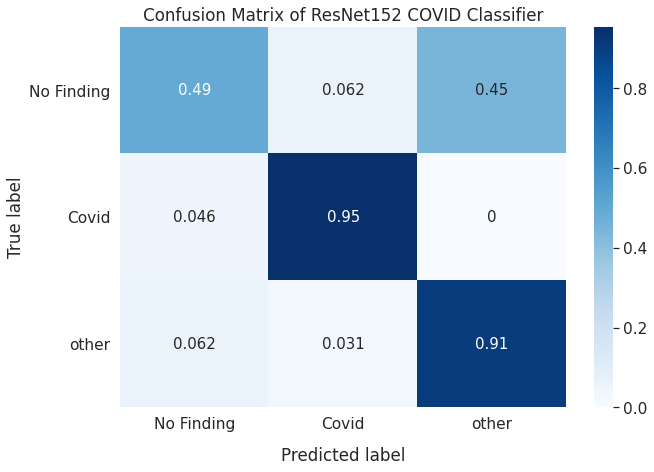
\includegraphics[width=0.75\textwidth]{../results/ResNet152_conf_matrix.png}
    \caption{}
\end{figure}

\section{SqueezeNet}

\begin{figure}[H]
    \centering
    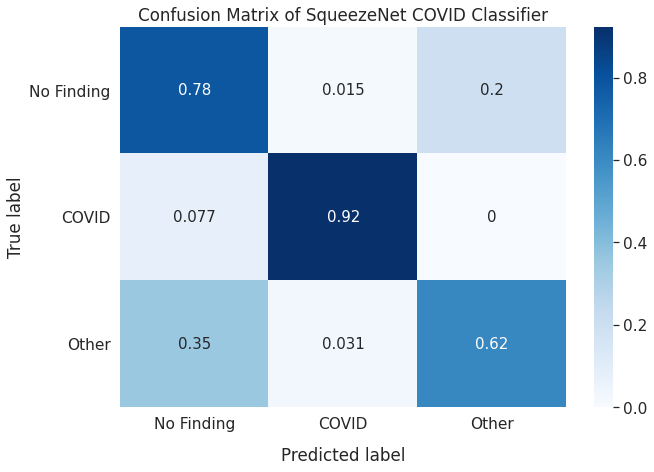
\includegraphics[width=0.75\textwidth]{../results/SqueezeNet_conf_matrix.png}
    \caption{}
\end{figure}

\begin{figure}[H]
    \centering
    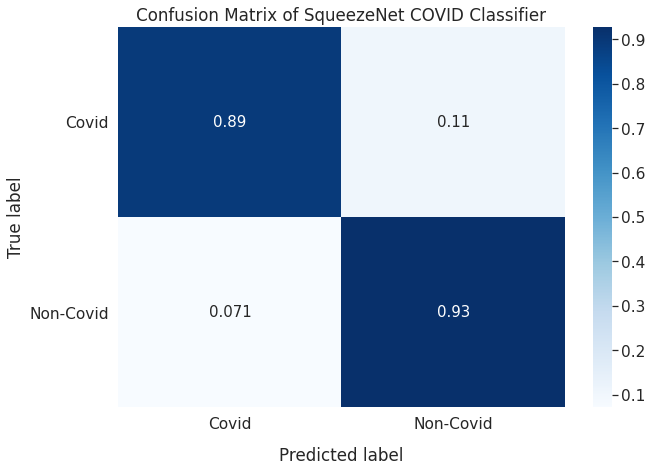
\includegraphics[width=0.75\textwidth]{../results/Binary_SqueezeNet_conf_matrix.png}
    \caption{}
\end{figure}